\section{Examples}
\label{sec:examples}

\subsection{Colors}

Here are some notable color variants:

\begin{enumerate}
	\item {\color{dkgreen} This is dkgreen.}
	\item {\color{deepgreen} This is deepgreen.}
	\item {\color{deepblue} This is deepblue.}
	\item {\color{darkorange} This is darkorange.}
	\item {\color{deepred} This is deepred.}
	\item {\color{lava} This is lava.}
\end{enumerate}

\subsection{Figures \& Tables}
In Fig. \ref{fig:figure} we see a graph. Table \ref{tab:test} shows the results.

\begin{figure}[h]
	\centering
	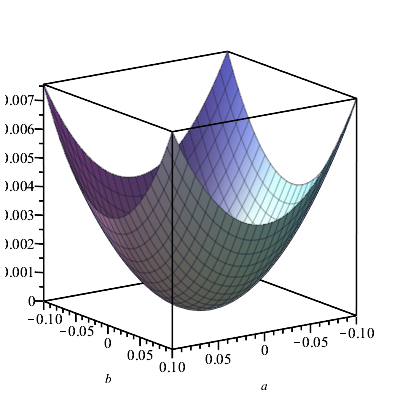
\includegraphics[width=5cm]{pictures/figure}
	\caption{This is some graph.}
	\label{fig:figure}
\end{figure}

\begin{table}[h]
	\begin{center}
		\begin{tabular}{|c|c|c|}
			\hline
			\backslashbox{hello}{world} & $T_1$ & $T_2$ \\
			\hline
			Test A & $0.25$ & $0.28$ \\
			\hline
			Test B & $0.19$ & $0.21$ \\
			\hline
		\end{tabular}
	\end{center}
	\caption{This is a test table.}
	\label{tab:test}
\end{table}

\subsection{Code}
You can also write code paragraphs, using the light theme

\begin{lstlisting}[language=Python]
	import numpy as np
	
	print(np.sum[1, 2, 3, 4, 5, 6, 7, 8, 9])
\end{lstlisting}

or the dark theme

\begin{lstlisting}[language=Python, style=dark]
	import numpy as np
	
	print(np.sum[1, 2, 3, 4, 5, 6, 7, 8, 9])
\end{lstlisting}

\subsection{New Commands}
$\bar{u}\tild{u}$

\subsection{Equations}
\begin{equation}
	e^{i\pi} = -1
\end{equation}

\begin{equation}
	\begin{split}
		Q(\lambda,\hat{\lambda}) = -\frac{1}{2} P{(O \mid \lambda )} \\\sum_s \sum_m \sum_t \gamma_m^{(s)} (t) \left( n \log(2 \pi ) + \log \left| C_m^{(s)} \right| + \left( \mathbf{o}_t - \hat{\mu}_m^{(s)} \right) ^T C_m^{(s)-1} \left(\mathbf{o}_t - \hat{\mu}_m^{(s)}\right) \right)
	\end{split}
\end{equation}